\nonstopmode

\documentclass[twoside,letterpaper]{article}
% \usepackage{a4}
\usepackage[latin1]{inputenc}
\usepackage[T1]{fontenc}
\usepackage{latexsym}
\usepackage{makeidx}
\usepackage{verbatim}

\usepackage{fancyhdr}

\usepackage{ifpdf}
\newif\ifpdf
\ifx\pdfoutput\undefined
\else
  \ifx\pdfoutput\relax
  \else
    \ifcase\pdfoutput
    \else
      \pdftrue
    \fi
  \fi
\fi
\ifpdf
  \usepackage[pdftex,colorlinks=true,bookmarksopen, pdfstartview=FitH,
              linkcolor=blue, citecolor=blue, urlcolor=blue]{hyperref}
  \usepackage[pdftex]{graphicx}
  \pdfcompresslevel=9
\else
  \usepackage[dvips]{graphicx}
\fi



\usepackage{ae}
\usepackage{aecompl}


% HORIZONTAL MARGINS
% Left margin, odd pages: 1.25 inch (0.25 + 1)
\setlength{\oddsidemargin}{0.25in}
% Left margin, even pages: 1.25 inch (0 + 1)
\setlength{\evensidemargin}{0.25in}
% Text width 6 inch (so other margin is 1.25 inch).
\setlength{\textwidth}{6in}
% ----------------
% VERTICAL MARGINS
% Top margin 0.5 inch (-0.5 + 1)
\setlength{\topmargin}{-0.5in}
% Head height 0.25 inch (where page headers go)
\setlength{\headheight}{0.25in}
% Head separation 0.25 inch (between header and top line of text)
\setlength{\headsep}{0.25in}
% Text height 9 inch (so bottom margin 1 in)
\setlength{\textheight}{9in}
% ----------------
% PARAGRAPH INDENTATION
\setlength{\parindent}{0in}
% SPACE BETWEEN PARAGRAPHS
\setlength{\parskip}{\medskipamount}
% ----------------
% STRUTS
% HORIZONTAL STRUT.  One argument (width).
\newcommand{\hstrut}[1]{\hspace*{#1}}
% VERTICAL STRUT. Two arguments (offset from baseline, height).
\newcommand{\vstrut}[2]{\rule[#1]{0in}{#2}}
% ----------------
% HORIZONTAL LINE ACROSS PAGE:
\newcommand{\hdivider}{\noindent\mbox{}\hrulefill\mbox{}} 
% ----------------
% EMPTY BOXES OF VARIOUS WIDTHS, FOR INDENTATION
\newcommand{\hm}{\hspace*{1em}}
\newcommand{\hmm}{\hspace*{2em}}
\newcommand{\hmmm}{\hspace*{3em}}
\newcommand{\hmmmm}{\hspace*{4em}}
% ----------------

\newcommand{\te}[1]{\texttt{#1}}

\newenvironment{libverbatim}
  {\vspace*{-1.0em}
   \verbatim}
  {\endverbatim
  }

% \title{
% {\BS}$^{\rm{TM}}$ {\SV} \\
% Version {\BSVVersion} \\
% Reference Guide \\
% \vspace*{1in}
% {\large\bf Please do not circulate without permission from Bluespec, Inc.} \\
% \vspace*{1in}
% \mbox{}
% }

%\input{../common_dates.tex}

\begin{document}

\section{TLM}
%\index{TLM (package)}
\label{sec-TLM}
%\index[bsvsource]{TLM}
%\index[bsvsource]{TLMCBusAdapter}
%\index[bsvsource]{TLMDefines}
%\index[bsvsource]{TLMRam}
%\index[bsvsource]{TLMReadWriteRam}
%\index[bsvsource]{TLMReduce}
%\index[bsvsource]{TLMUtils}

{\bf Packages}

\begin{verbatim}
import TLM :: * ;
\end{verbatim}




{\bf Description}
 
The TLM package includes definitions of interfaces, data structures,
and module constructors which allow users to create and modify
bus-based designs in a manner that is independent of any one specific
bus protocol. Bus operations are defined in terms of generic bus
payload data structures. Other protocol specific packages include
transactor modules that convert a stream of TLM bus operations into
corresponding operations in a specific bus protocol. Designs created
using the TLM package are thus more portable (because that they allow
the core design to be easily applied to multiple bus protocols). In
addition, since the specific signalling details of each bus protocol
are encapsulated in pre-designed transactors, users are not required
to learn, re-implement, and re-verify existing standard protocols.

%\input{source}


{\bf Data Structures}
\label{TLM-data}
 
The two basic data structures defined in the \te{TLM} package are
\te{TLMRequest} and \te{TLMResponse}.  By using these
types in a design, the underlying bus protocol
can be changed without having to modify the interactions with the
\te{TLM} objects.


\paragraph{\bf TLMRequest}
%\index{TLMRequest@\te{TLMRequest} (data structure)}

%\index{RequestData@\te{RequestData} (data structure)}


A TLM request contains either control information and data, or data
alone.  A \te{TLMRequest} is tagged as either a  \te{RequestDescriptor} or
\te{RequestData}.   A \te{RequestDescriptor} contains
control information and data while a \te{RequestData} 
contains only  data.


\begin{verbatim}
typedef union tagged {RequestDescriptor#(`TLM_TYPES) Descriptor;
                      RequestData#(`TLM_TYPES) Data;       
                     } TLMRequest#(`TLM_TYPE_PRMS) deriving(Eq, Bits, Bounded);
\end{verbatim} 

\begin{verbatim}
typedef TLMRequest#(`TLM_STD_TYPES)  TLMRequestStd;
\end{verbatim}

\paragraph{RequestDescriptor}
%\index{RequestDescriptor@\te{RequestDescriptor} (data structure)}
The table below describes the components of a
\te{RequestDescriptor}  and  the valid values for each of its members.


\begin{center}
\begin{tabular}{|p{1.2 in}|p{2in}|p{3in}|}
\hline
\multicolumn{3}{|c|}{RequestDescriptor} \\
\hline
\multicolumn{1}{|c|}{Member Name}&\multicolumn{1}{|c|}{DataType}&\multicolumn{1}{|c|}{Valid Values} \\
\hline
\hline
\te{command}&\te{TLMCommand}&READ, WRITE, UNKNOWN\\
\hline
\te{mode}&\te{TLMMode}&REGULAR, DEBUG, CONTROL\\
\hline
\te{addr}&\te{TLMAddr\#(`TLM\_TYPES)}&\te{Bit\#(addr\_size)}\\
\hline
\te{data}&\te{TLMData\#(`TLM\_TYPES)}&\te{Bit\#(data\_size)}\\
\hline
\te{burst\_length}&\te{TLMUint\#(`TLM\_TYPES)}&\te{UInt\#(uint\_size)}\\
\hline
\te{byte\_enable}&\te{TLMByteEn\#(`TLM\_TYPES)}&\te{Bit\#(TDiv\#(data\_size,
8))}\\
\hline
\te{burst\_mode}&\te{TLMBurstMode}&INCR, CNST, WRAP, UNKNOWN\\
\hline
\te{burst\_size}&\te{TLMBurstSize\#(`TLM\_TYPES)}&\te{Bit\#(TLog\#(TDiv\#(data\_size,
8)))}\\
\hline
\te{prty}&\te{TLMUInt\#(`TLM\_TYPES)}&\te{UInt\#(uint\_size)}\\
\hline
\te{lock}&\te{Bool}&\\
\hline
\te{thread\_id}&\te{TLMId\#(`TLM\_TYPES)}&\te{Bit\#(id\_size)}\\
\hline
\te{transaction\_id}&\te{TLMId\#(`TLM\_TYPES)}&\te{Bit\#(id\_size)}\\
\hline
\te{export\_id}&\te{TLMId\#(`TLM\_TYPES)}&\te{Bit\#(id\_size)}\\
\hline
\te{custom}&\te{TLMCustom\#(`TLM\_TYPES)}&\te{cstm\_type}\\
\hline
\end{tabular}
\end{center}

\begin{verbatim}
typedef struct {TLMCommand                command;
                TLMMode                   mode;
                TLMAddr#(`TLM_TYPES)      addr;
                TLMData#(`TLM_TYPES)      data;
                TLMUInt#(`TLM_TYPES)      burst_length;
                TLMByteEn#(`TLM_TYPES)    byte_enable;
                TLMBurstMode              burst_mode;
                TLMBurstSize#(`TLM_TYPES) burst_size;
                TLMUInt#(`TLM_TYPES)      prty;
                Bool                      lock;
                TLMId#(`TLM_TYPES)        thread_id;
                TLMId#(`TLM_TYPES)        transaction_id;
                TLMId#(`TLM_TYPES)        export_id;
                TLMCustom#(`TLM_TYPES)    custom;
                } RequestDescriptor#(`TLM_TYPE_PRMS) deriving (Eq, Bits, Bounded);
\end{verbatim}


%\index{RequestData@\te{RequestData} (data structure)}
\paragraph{RequestData} The table below describes the components of a
                \te{RequestData}  and the valid values for its members.

\begin{center}
\begin{tabular}{|p{1.2 in}|p{2 in}|p{3in}|}
\hline
\multicolumn{3}{|c|}{RequestData} \\
\hline
\multicolumn{1}{|c|}{Member Name}&\multicolumn{1}{|c|}{DataType}&\multicolumn{1}{|c|}{Valid Values} \\
\hline
\hline
\te{data}&\te{TLMData\#(`TLM\_TYPES)}&\te{Bit\#(data\_size)}\\
\hline
\te{transaction\_id}&\te{TLMId\#(`TLM\_TYPES)}&\te{Bit\#(id\_size)}\\
\hline
\te{custom}&\te{TLMCustom\#(`TLM\_TYPES)}&\te{cstm\_type}\\
\hline
\end{tabular}
\end{center}


\begin{verbatim}
typedef struct {TLMData#(`TLM_TYPES)   data;
                TLMId#(`TLM_TYPES)     transaction_id;
                TLMCustom#(`TLM_TYPES) custom;
               } RequestData#(`TLM_TYPE_PRMS) deriving (Eq, Bits, Bounded);
\end{verbatim}



\paragraph{\bf TLMResponse}  The table below describes the components of a
                \te{TLMResponse}  and the valid values for its members.
%\index{TLMResponse@\te{TLMResponse} (data structure)}


\begin{center}
\begin{tabular}{|p{1.2 in}|p{2 in}|p{3in}|}
\hline
\multicolumn{3}{|c|}{TLMResponse} \\
\hline
\multicolumn{1}{|c|}{Member Name}&\multicolumn{1}{|c|}{DataType}&\multicolumn{1}{|c|}{Valid Values} \\
\hline
\hline
\te{command}&\te{TLMCommand}&READ, WRITE, UNKNOWN\\
\hline
\te{data}&\te{TLMData\#(`TLM\_TYPES)}&\te{Bit\#(data\_size)}\\
\hline
\te{status}&\te{TLMStatus}&SUCCESS, ERROR, NO\_RESPONSE\\
\hline
\te{prty}&\te{TLMUInt\#(`TLM\_TYPES)}&\te{UInt\#(uint\_size)}\\
\hline
\te{thread\_id}&\te{TLMId\#(`TLM\_TYPES)}&\te{Bit\#(id\_size)}\\
\hline
\te{transaction\_id}&\te{TLMId\#(`TLM\_TYPES)}&\te{Bit\#(id\_size)}\\
\hline
\te{export\_id}&\te{TLMId\#(`TLM\_TYPES)}&\te{Bit\#(id\_size)}\\
\hline
\te{custom}&\te{TLMCustom\#(`TLM\_TYPES)}&\te{cstm\_type}\\
\hline
\end{tabular}
\end{center}


\begin{verbatim}
typedef struct {TLMCommand             command;
                TLMData#(`TLM_TYPES)   data;
                TLMStatus              status;
                TLMUInt#(`TLM_TYPES)   prty;
                TLMId#(`TLM_TYPES)     thread_id;
                TLMId#(`TLM_TYPES)     transaction_id;
                TLMId#(`TLM_TYPES)     export_id;
                TLMCustom#(`TLM_TYPES) custom;
                } TLMResponse#(`TLM_TYPE_PRMS) deriving (Eq, Bits, Bounded);
\end{verbatim}

\begin{verbatim}
typedef TLMResponse#(`TLM_STD_TYPES) TLMResponseStd;
\end{verbatim}


{\bf Configurable Parameters}
\label{TLM-defines}
%\index{TLM.defines@\te{TLM.defines}}
%\index{TLM\_TYPE\_PRMS@\te{TLM\_TYPE\_PRMS}}
%\index{TLM\_TYPE@\te{TLM\_TYPE}}
%\index{TLM\_STD\_TYPES@\te{TLM\_STD\_TYPES}}

 
In the above BSV code definitions the compiler macros
 \te{`TLM\_TYPE\_PRMS} and \te{`TLM\_TYPES} are used in the
\te{typedef} statements.  A \te{'define} statement is a preprocessor
 construct used to place prepackaged text values into a file.  In this case, the  macros
 contain   parameters to be used in the
 data definitions.  Placing the  parameters in a separate file allows them
 to be easily modified for different protocol requirements.  For
 convenience, we have predefined a few useful definitions for use in
 the TLM package.

The \te{TLM\_TYPE\_PRMS} macro contains type definition parameters
which are used in the interface definitions or as arguments to TLM
types and interfaces.

The \te{TLM\_TYPES} macro is used when providing the interface or
using the data type. \te{TLM\_TYPES} is still polymorphic.

The macro \te{TLM\_STD\_TYPES} provides specific values for the
polymorphic values defined above. The values defined in
\te{TLM\_STD\_TYPES} are common values. The user can change any of the
values or define other corresponding macros (with different values) as
appropriate for a given design.

The macros  are found in the file \te{TLM.defines}.  A
sample of the  contents of the file are displayed below.

\begin{verbatim}
`define TLM_TYPE_PRMS numeric type id_size, numeric type addr_size, \
                      numeric type data_size, numeric type uint_size, type cstm_type
`define TLM_TYPES id_size, addr_size, data_size, uint_size, cstm_type
`define TLM_STD_TYPES  4, 32, 32, 10, Bit#(0)
\end{verbatim}


{\bf Interfaces}
%\index{TLMRecvIFC@\te{TLMRecvIFC} (interface)}
%\index{TLMSendIFC@\te{TLMSendIFC} (interface)}
 
\label{TLM-interfaces}
% Interfaces in Bluespec  encapsulate interconnect and communication
% thus  separating communication from functionality and enabling
% abstraction  in the design. 
The TLM interfaces define how TLM blocks interconnect and communicate.
The TLM package includes two basic interfaces: The \te{TLMSendIFC}
interface and the \te{TLMRecvIFC} interface.  These interfaces use 
basic \te{Get} and \te{Put} subinterfaces as the requests and responses. The \te{TLMSendIFC} interface
generates (\te{Get}) requests  and receives (\te{Put}) responses. 
The \te{TLMRecvIFC} interface receives (\te{Put}) requests and
generates (\te{Get}) responses. Additional TLM interfaces are built up from
these basic blocks.


\paragraph{\bf TLMSendIFC}
The \te{TLMSendIFC} interface transmits the requests and receives the
responses.

% is used for generating requests.  The interface
% gets the request and puts the response .  
% The \te{TLMSendIFC} two sub-interfaces, \te{tx} to \te{Get} the
% request and \te{Rx} to put the response.


\begin{center}
\begin{tabular}{|p{.5 in}|p{2.5 in}|p{3 in}|}
\hline
\multicolumn{3}{|c|}{TLMSendIFC Interface}\\
\hline
Name & Type & Description \\
\hline
\hline 
\te{tx}  &\te{Get\#(TLMRequest\#(`TLM\_TYPES))}  &Transmits a request
through the \te{Get} interface \\
\hline
\te{rx}  &\te{Put\#(TLMResponse\#(`TLM\_TYPES))}  &Receives a response
through the \te{Put} interface\\
\hline
\end{tabular}
\end{center}


\begin{verbatim}
    interface TLMSendIFC#(`TLM_TYPE_PRMS);
       interface Get#(TLMRequest#(`TLM_TYPES))  tx;
       interface Put#(TLMResponse#(`TLM_TYPES)) rx;
    endinterface
\end{verbatim}


\paragraph{\bf TLMRecvIFC}
The \te{TLMRecvIFC} interface receives the requests and transmits the responses.

\begin{center}
\begin{tabular}{|p{.5 in}|p{2.5 in}|p{3 in}|}
\hline
\multicolumn{3}{|c|}{TLMRecvIFC Interface}\\
\hline
Name & Type & Description \\
\hline
\hline 
\te{tx}  &\te{Get\#(TLMResponse\#(`TLM\_TYPES))}  &Transmits the
response through the \te{Get} interface\\
\hline
\te{rx}  &\te{Put\#(TLMRequest\#(`TLM\_TYPES))}  &Receives the request
through the \te{Put} interface\\
\hline
\end{tabular}
\end{center}

\begin{verbatim}
    interface TLMRecvIFC#(`TLM_TYPE_PRMS);
       interface Get#(TLMResponse#(`TLM_TYPES)) tx;
       interface Put#(TLMRequest#(`TLM_TYPES))  rx;
    endinterface
\end{verbatim}


As illustrated in Figure \ref{TLMconnect}, a \te{TLMSendIFC} is
connectable to a \te{TLMRecvIFC}, just as a \te{Get} is connectable to
a \te{Put}.  A transmitted request (\te{tx})
from a \te{TLMSendIFC} is received (\te{rx}) by the \te{TLMRecvIFC}
and visa versa.

\begin{figure}[ht]
\begin{center}
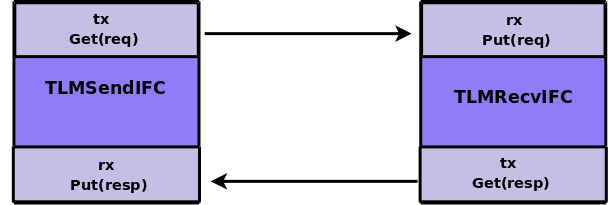
\includegraphics[height = 1.2 in]{TLMinterfaces}
\caption{Connecting TLM Send And Receive Interfaces}
\label{TLMconnect}
\end{center}
\end{figure}


\begin{verbatim}
instance Connectable#(TLMSendIFC#(`TLM_TYPES), TLMRecvIFC#(`TLM_TYPES));
\end{verbatim}

%% \begin{verbatim}
%%     instance Connectable#(TLMSendIFC#(`TLM_TYPES), TLMRecvIFC#(`TLM_TYPES));
%%        module mkConnection#(TLMSendIFC#(`TLM_TYPES) request, 
%%                             TLMRecvIFC#(`TLM_TYPES) response) (Empty);
%%           mkConnection(request.tx, response.rx);
%%           mkConnection(request.rx, response.tx);
%%        endmodule
%%     endinstance
%% \end{verbatim}

A module with a \te{TLMSendIFC} interface creates a stream of
requests. A module with a \te{TLMRecvIFC} interface receives the
requests and transmits responses. Some bus protocols have separate
channels for read and write operations. In these cases it is useful to
have interfaces which bundle together two sends or two receives.  The
\te{TLMReadWriteSendIFC} interface includes two send interfaces while
the \te{TLMReadWriteRecvIFC} interface bundles two receives.


\paragraph{\bf TLMReadWriteSendIFC}
%\index{TLMReadWriteSendIFC@\te{TLMReadWriteSendIFC} (interface)}

The \te{TLMReadWriteSendIFC} interface is composed of two
\te{TLMSendIFC} subinterfaces, one for a read channel and one for a
write channel.

\begin{verbatim}
    interface TLMReadWriteSendIFC#(`TLM_TYPE_PRMS);
       interface TLMSendIFC#(`TLM_TYPES) read;
       interface TLMSendIFC#(`TLM_TYPES) write;
    endinterface
\end{verbatim}

\paragraph{\bf TLMReadWriteRecvIFC}
%\index{TLMReadWriteRecvIFC@\te{TLMReadWriteRecvIFC} (interface)}

The \te{TLMReadWriteRecvIFC} interface is composed of two
\te{TLMRecvIFC} subinterfaces, one for a read channnel and one for a
write channel.

\begin{verbatim}
    interface TLMReadWriteRecvIFC#(`TLM_TYPE_PRMS);
       interface TLMRecvIFC#(`TLM_TYPES) read;
       interface TLMRecvIFC#(`TLM_TYPES) write;
    endinterface
\end{verbatim}

As illustrated in Figure \ref{TLMrwinterface}, the \te{TLMReadWriteSendIFC} and 
\te{TLMReadWriteRecvIFC} interfaces are connectable as well.

\begin{figure}[ht]
\begin{center}
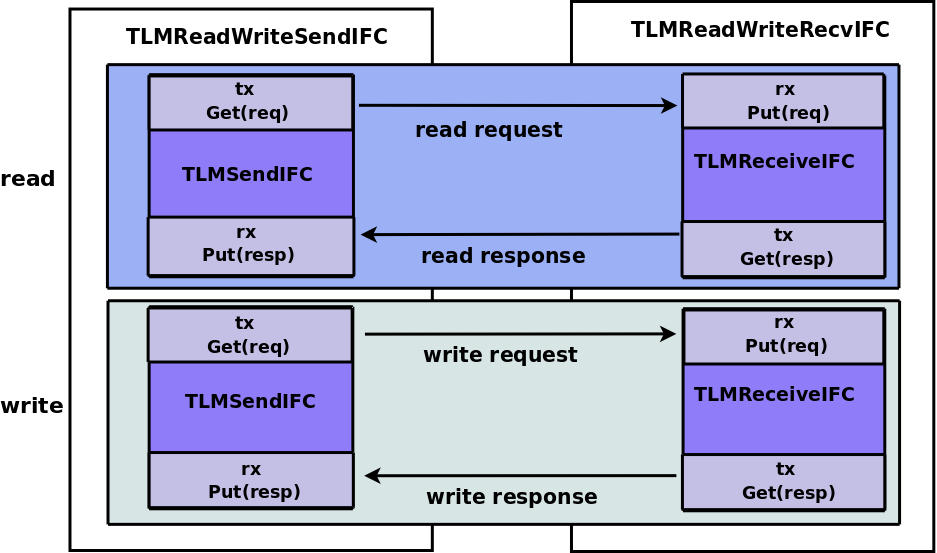
\includegraphics[height = 2.4 in]{TLMrwinterfaces}
\caption{TLM Read/Write Interfaces}
\label{TLMrwinterface}
\end{center}
\end{figure}


\begin{verbatim}
instance Connectable#(TLMReadWriteSendIFC#(`TLM_TYPES), TLMReadWriteRecvIFC#(`TLM_TYPES));
\end{verbatim}

%% \begin{verbatim}
%%     instance Connectable#(TLMReadWriteSendIFC#(`TLM_TYPES), TLMReadWriteRecvIFC#(`TLM_TYPES));
%%        module mkConnection#(TLMReadWriteSendIFC#(`TLM_TYPES) request, 
%%                             TLMReadWriteRecvIFC#(`TLM_TYPES) response) (Empty);
%%           let read_con  <- mkConnection(request.read,  response.read);
%%           let write_con <- mkConnection(request.write, response.write);
%%        endmodule
%%     endinstance
%% \end{verbatim}


\paragraph{TLMTransformIFC}
%\index{TLMTransformIFC@\te{TLMTransformIFC} (interface)}

The \te{TLMTransformIFC} provides a single \te{TLMRecvIFC} interface
and a single \te{TLMSendIFC} interface. This interface is useful in
modules which convert one stream of TLM operations into another. It is 
the interface provided by \te{mkTLMReducer} module for instance.

\begin{figure}[ht]
\begin{center}
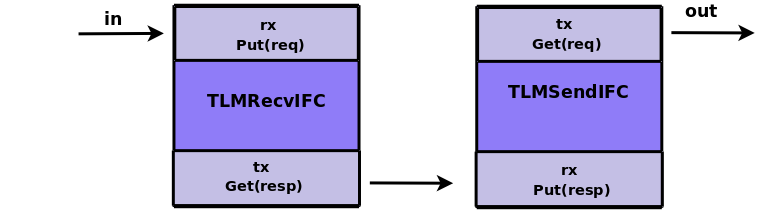
\includegraphics[height = 1.2 in]{TLMTransformIFC}
\caption{TLMTransformIFC Interface}
\label{TLMtransform}
\end{center}
\end{figure}


\begin{verbatim}
    interface TLMTransformIFC#(`TLM_TYPE_PRMS);
       interface TLMRecvIFC#(`TLM_TYPES) in;
       interface TLMSendIFC#(`TLM_TYPES) out;
    endinterface
\end{verbatim}

{\bf Modules}
 
\label{sec-TLM-modules}
%\index{mkTLMRandomizer@\te{mkTLMRandomizer} (module)}
%\index{mkTLMSource@\te{mkTLMSource} (module)}
%\index{mkTLMReducer@\te{mkTLMReducer} (module)}
%\index{mkTLMRam@\te{mkTLMRam} (module)}
%\index{mkTLMReadWriteRam@\te{mkTLMReadWriteRam} (module)}
%\index[function]{TLM!mkTLMRandomizer}
%\index[function]{TLM!mkTLMSource}
%\index[function]{TLM!mkTLMReducer}
%\index[function]{TLM!mkTLMRam}
%\index[function]{TLM!mkTLMReadWriteRam}

The TLM package includes modules for creating and modifying TLM
objects: \te{mkTLMRandomizer}, \te{mkTLMSource}, and
\te{mkTLMReducer}.  Two TLM RAM modules are also provided:
\te{mkTLMRam} which provides a single read/write port and
\te{mkTLMReadWriteRam} which provides two ports, a separate one for
reads and a separate one for writes.

\begin{center}
\begin{tabular}{|p{1.2 in}|p{5 in}|}
\hline 
&\\
\te{mkTLMRandomizer}&Creates a stream of random TLM
operations.  The argument \te{m\_command} is a \te{Maybe} type which
determines if the \te{TLMRequest}s will be reads, writes, or both. A
value of \te{Valid READ} will generate only reads, a value of
\te{Valid WRITE} will generate only writes, and an \te{Invalid} value will
generate both reads and writes. The \te{Randomize} interface is
defined in the \te{Randomizable} package. \\
&\\
\cline{2-2}
&\begin{libverbatim}
module mkTLMRandomizer#(Maybe#(TLMCommand) m_command) 
                       (Randomize#(TLMRequest#(`TLM_TYPES)))
   provisos(Bits#(RequestDescriptor#(`TLM_TYPES), s0),
            Bounded#(RequestDescriptor#(`TLM_TYPES)),
            Bits#(RequestData#(`TLM_TYPES), s1),
            Bounded#(RequestData#(`TLM_TYPES)));
\end{libverbatim}
\\
\hline
\end{tabular}
\end{center}

\begin{center}
\begin{tabular}{|p{1.2 in}|p{5 in}|}
\hline 
&\\
\te{mkTLMSource}&Creates a wrapper around the \te{mkTLMRandomize} module.
The provided interface is now a \te{TLMSendIFC} interface which both
sends \te{TLMRequest}s and receives \te{TLMResponse}s. The argument
\te{m\_command} has the same meaning as in \te{mkTLMRandomizer}. The \te{verbose} 
argument controls whether or not  \te{\$display} outputs are provide when
sending and receiving TLM objects. \\
&\\
\cline{2-2}
&\begin{libverbatim}
module mkTLMSource#(Maybe#(TLMCommand) m_command, Bool verbose) 
                   (TLMSendIFC#(`TLM_STD_TYPES));
\end{libverbatim}
\\
\hline
\end{tabular}
\end{center}

\begin{center}
\begin{tabular}{|p{1.2 in}|p{5 in}|}
\hline 
&\\
\te{mkTLMReducer}&Converts a stream of (arbitrary) TLM
operations into a stream with only single reads and single writes.\\
&\\
\cline{2-2}
&\begin{libverbatim}
module mkTLMReducer (TLMTransformIFC#(`TLM_TYPES))
   provisos(Bits#(TLMRequest#(`TLM_TYPES), s0),
            Bits#(TLMResponse#(`TLM_TYPES), s1),
            Bits#(RequestDescriptor#(`TLM_TYPES), s2));
\end{libverbatim}
\\
\hline
\end{tabular}
\end{center}

\begin{figure}[ht]
\begin{center}
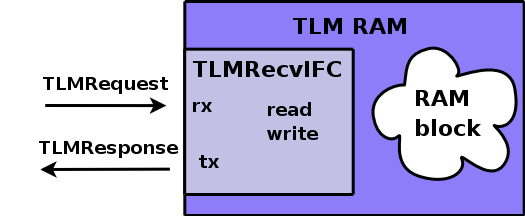
\includegraphics[height = .8 in]{TLMRAM}
\caption{TLMRAM}
\label{ram}
\end{center}
\end{figure}

\begin{center}
\begin{tabular}{|p{1.2 in}|p{5 in}|}
\hline 
&\\
\te{mkTLMRam}&Creates a TLM RAM with a single port for read
and write operations.  Provides the \te{TLMRecvIFC} interface.  The
\te{verbose} argument controls whether or not \te{\$display} output
is provided when performing a memory operation. The \te{id} argument
provides an identifier for the instantiation which is used in the
\te{\$display} output if the \te{verbose} flag is asserted. \\ 
&\\
\cline{2-2}
&\begin{libverbatim}
module mkTLMRam#(parameter Bit#(4) id, Bool verbose) 
                (TLMRecvIFC#(`TLM_TYPES))
   provisos(Bits#(TLMRequest#(`TLM_TYPES),  s0),
            Bits#(TLMResponse#(`TLM_TYPES), s1));
\end{libverbatim}
\\
\hline
\end{tabular}
\end{center}

\begin{figure}[ht]
\begin{center}
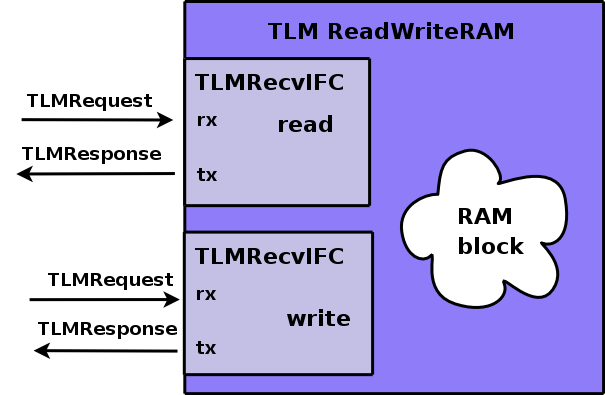
\includegraphics[height = 1.5 in]{TLMReadWriteRAM}
\caption{TLMReadWriteRAM}
\label{rwram}
\end{center}
\end{figure}


\begin{center}
\begin{tabular}{|p{1.2 in}|p{5 in}|}
\hline 
&\\

\te{mkTLMReadWriteRam}&Creates a RAM with separate ports for read 
and write operations.  Provides the \te{TLMReadWriteRecvIFC}
interface. The \te{verbose} argument controls whether or not
\te{\$display} output is provided when performing a memory
operation. The \te{id} argument provides an identifier for the
instantiation which is used in the \te{\$display} output if the
\te{verbose} flag is asserted. \\
&\\
\cline{2-2}
&\begin{libverbatim}
module mkTLMReadWriteRam#(parameter Bit#(4) id, Bool verbose) 
                         (TLMReadWriteRecvIFC#(`TLM_TYPES))
   provisos(Bits#(TLMRequest#(`TLM_TYPES),  s0),
            Bits#(TLMResponse#(`TLM_TYPES), s1));
\end{libverbatim}
\\
\hline
\end{tabular}
\end{center}

The \te{mkTLMCBusAdapter} module creates an adapter which allows the
\te{CBus} to be accessed via a TLM interface.

\begin{center}
\begin{tabular}{|p{1.2 in}|p{5 in}|}
\hline 
&\\
\te{mkTLMCBusAdapter}&Takes a \te{TLMCBus} interface as an argument.
Provides the \te{TLMRecvIFC} interface. \\ 
&\\
\cline{2-2}
&\begin{libverbatim}
module mkTLMCBusAdapter#(TLMCBus#(`TLM_TYPES, caddr_size) cfg)
                        (TLMRecvIFC#(`TLM_TYPES))
   provisos(Bits#(TLMRequest#(`TLM_TYPES),  s0),
	    Bits#(TLMResponse#(`TLM_TYPES), s1),
	    Add#(ignore, caddr_size, addr_size));
\end{libverbatim}
\\
\hline
\end{tabular}
\end{center}




\begin{center}
\begin{tabular}{|p{2 in}|p{4.2 in}|}
\hline 
%\multicolumn{2}{|l|}{\te{mkTLMCBusAdapterToReadWrite}} \\ 
&\\
\te{mkTLMCBusAdapterToReadWrite}&Takes a \te{TLMCBus} interface as an argument.
Provides the \te{TLMReadWriteRecvIFC} interface. This configuration provides 
separate ports for read and write operations.\\ 
&\\
\cline{2-2}
&\begin{libverbatim}
module mkTLMCBusAdapterToReadWrite#
                  (TLMCBus#(`TLM_TYPES, caddr_size) cfg)
                  (TLMReadWriteRecvIFC#(`TLM_TYPES))
   provisos(Bits#(TLMRequest#(`TLM_TYPES),  s0),
	    Bits#(TLMResponse#(`TLM_TYPES), s1),
	    Add#(ignore, caddr_size, addr_size));
\end{libverbatim}
\\
\hline
\end{tabular}
\end{center}


{\bf Functions}


% \begin{center}
% \begin{tabular}{|p{1.2 in}|p{5 in}|}
% \hline 
% &\\
% \te{}& \\ 
% &\\
% \cline{2-2}
% &\begin{libverbatim}
% \end{libverbatim}
% \\
% \hline
% \end{tabular}
% \end{center}

% \begin{center}
% \begin{tabular}{|p{1.2 in}|p{5 in}|}
% \hline 
% &\\
% \te{getTLMCycleCount}& \\ 
% &\\
% \cline{2-2}
% &\begin{libverbatim}
% function TLMUInt#(`TLM_TYPES) 
%          getTLMCycleCount (RequestDescriptor#(`TLM_TYPES) desc);
% \end{libverbatim}
% \\
% \hline
% \end{tabular}
% \end{center}


% \begin{center}
% \begin{tabular}{|p{1.2 in}|p{5 in}|}
% \hline 
% &\\
% \te{getTLMBurstSize}&Returns the size of the burst as a \te{Bit\#(n)}. \\ 
% &\\
% \cline{2-2}
% &\begin{libverbatim}
% function Bit#(n) getTLMBurstSize (RequestDescriptor#(`TLM_TYPES) desc)
%    provisos(Add#(SizeOf#(TLMBurstSize#(`TLM_TYPES)), 1, n));
% \end{libverbatim}
% \\
% \hline
% \end{tabular}
% \end{center}


% \begin{center}
% \begin{tabular}{|p{1.2 in}|p{5 in}|}
% \hline 
% &\\
% \te{getTLMIncr}&Returns the TLM increment as a \te{Bit\#(n)}. \\ 
% &\\
% \cline{2-2}
% &\begin{libverbatim}
% function Bit#(n) getTLMIncr (RequestDescriptor#(`TLM_TYPES) desc)
%    provisos(Add#(SizeOf#(TLMBurstSize#(`TLM_TYPES)), 1, n));
% \end{libverbatim}
% \\
% \hline
% \end{tabular}
% \end{center}


% \begin{center}
% \begin{tabular}{|p{1.2 in}|p{5 in}|}
% \hline 
% &\\
% \te{incrTLMAddr}&Returns a TLM Address. \\ 
% &\\
% \cline{2-2}
% &\begin{libverbatim}
% function RequestDescriptor#(`TLM_TYPES) 
%          incrTLMAddr(RequestDescriptor#(`TLM_TYPES) desc);
% \end{libverbatim}
% \\
% \hline
% \end{tabular}
% \end{center}


% \begin{center}
% \begin{tabular}{|p{1.2 in}|p{5 in}|}
% \hline 
% &\\
% \te{incrTLMAddrAV}& \\ 
% &\\
% \cline{2-2}
% &\begin{libverbatim}
% function ActionValue#(RequestDescriptor#(`TLM_TYPES)) 
%          incrTLMAddrAV(RequestDescriptor#(`TLM_TYPES) desc);
% \end{libverbatim}
% \\
% \hline
% \end{tabular}
% \end{center}

% \begin{center}
% \begin{tabular}{|p{1.2 in}|p{5 in}|}
% \hline 
% &\\
% \te{countLSBZeros}& \\ 
% &\\
% \cline{2-2}
% &\begin{libverbatim}
% function Bit#(n) countLSBZeros (Bit#(n) value);
% \end{libverbatim}
% \\
% \hline
% \end{tabular}
% \end{center}
    
% \begin{center}
% \begin{tabular}{|p{1.2 in}|p{5 in}|}
% \hline 
% &\\
% \te{getTLMData}&Returns the data from a TLM request. \\ 
% &\\
% \cline{2-2}
% &\begin{libverbatim}
% function TLMData#(`TLM_TYPES) 
%          getTLMData(TLMRequest#(`TLM_TYPES) request);
% \end{libverbatim}
% \\
% \hline
% \end{tabular}
% \end{center}


\begin{center}
\begin{tabular}{|p{2 in}|p{4.2 in}|}
\hline 
&\\
\te{createBasicRequestDescriptor}&Returns a generic TLM request
with default values. \\ 
&\\
\cline{2-2}
&\begin{libverbatim}
function RequestDescriptor#(`TLM_TYPES) 
         createBasicRequestDescriptor()
   provisos(Bits#(RequestDescriptor#(`TLM_TYPES), s0));
\end{libverbatim}
\\
\hline
\end{tabular}
\end{center}


\begin{center}
\begin{tabular}{|p{1.6 in}|p{4.6 in}|}
\hline 
&\\
\te{createBasicTLMResponse}& Returns a generic TLM response
with default values.\\ 
&\\
\cline{2-2}
&\begin{libverbatim}
function TLMResponse#(`TLM_TYPES) createBasicTLMResponse()
   provisos(Bits#(TLMResponse#(`TLM_TYPES), s0));
\end{libverbatim}
\\
\hline
\end{tabular}
\end{center}


% \begin{center}
% \begin{tabular}{|p{1.2 in}|p{5 in}|}
% \hline 
% &\\
% \te{createTLMBitMask}& \\ 
% &\\
% \cline{2-2}
% &\begin{libverbatim}
% function TLMData#(`TLM_TYPES) 
%          createTLMBitMask (TLMByteEn#(`TLM_TYPES) enable_bits);
% \end{libverbatim}
% \\
% \hline
% \end{tabular}
% \end{center}


% \begin{center}
% \begin{tabular}{|p{1.2 in}|p{5 in}|}
% \hline 
% &\\
% \te{maskTLMData}& \\ 
% &\\
% \cline{2-2}
% &\begin{libverbatim}
% function TLMData#(`TLM_TYPES) 
%          maskTLMData(TLMByteEn#(`TLM_TYPES) byte_enable, 
%                      TLMData#(`TLM_TYPES) data);
% \end{libverbatim}
% \\
% \hline
% \end{tabular}
% \end{center}


% \begin{center}
% \begin{tabular}{|p{1.2 in}|p{5 in}|}
% \hline 
% &\\
% \te{overwriteTLMData}& \\ 
% &\\
% \cline{2-2}
% &\begin{libverbatim}
% function TLMData#(`TLM_TYPES) 
%          overwriteTLMData(TLMByteEn#(`TLM_TYPES) byte_enable, 
%                           TLMData#(`TLM_TYPES) data_orig, 
%                           TLMData#(`TLM_TYPES) data);
% \end{libverbatim}
% \\
% \hline
% \end{tabular}
% \end{center}

   
\end{document}
